% !TEX root = ../SYSprojektrapport.tex
% SKAL STÅ I TOPPEN AF ALLE FILER FOR AT MASTER-filen KOMPILERES 

% !TEX root = ../SYSprojektrapport.tex
% SKAL STÅ I TOPPEN AF ALLE FILER FOR AT MASTER-filen KOMPILERES 

\label{ResultatOgDiskussion2}

\section{Case 2: Husstandsbatteriers evne til at absorbere overproduktion}
I dette afsnit præsenteres resultater for simuleringen af case 2 iht. beskrivelsen i afsnit \ref{SimCase2}. I de 2 tilstande er spændingsændringen ved Town5 busbar (rød linje) og Transmission central 60kV busbar (Grøn linje) samt frekvensændringen på Transmission central 60kV busbar (Grøn linje), præsenteret på hhv. spændingsgraf og frekvensgraf. Derudover er der lavet opsamling over spænding samt effektoverførelse andre relevante steder i systemet i tabel \ref{fig:C2Overview}. \\ \\

\textbf{Tilstand 1: Alle batterierne er frakoblet.}
\begin{figure}[H]
	\centering
	\begin{minipage}[b]{0.48\textwidth}
		\centering
		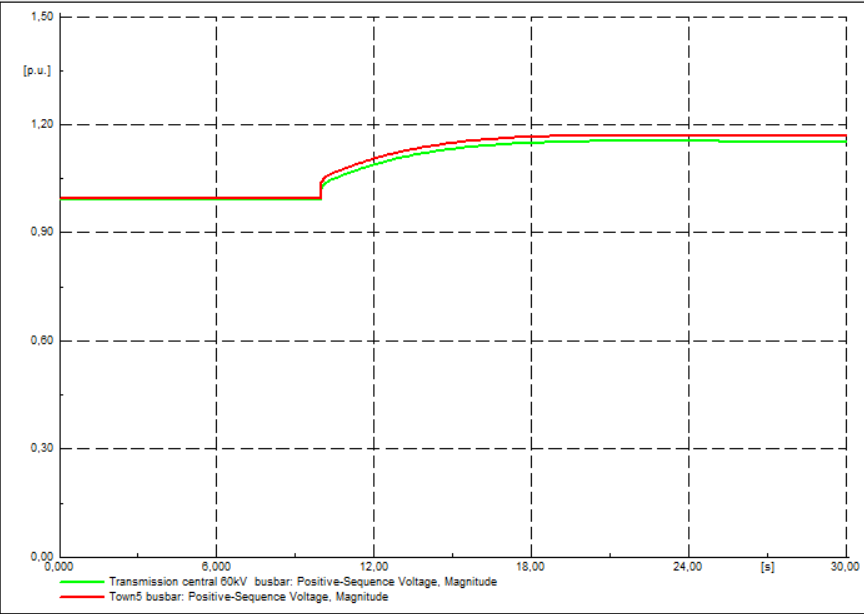
\includegraphics[width=1.00\textwidth]{figurer/LossOfTown/Voltage1} % Venstre billede
	\end{minipage}
	\hfill
	\begin{minipage}[b]{0.48\textwidth}
		\centering
		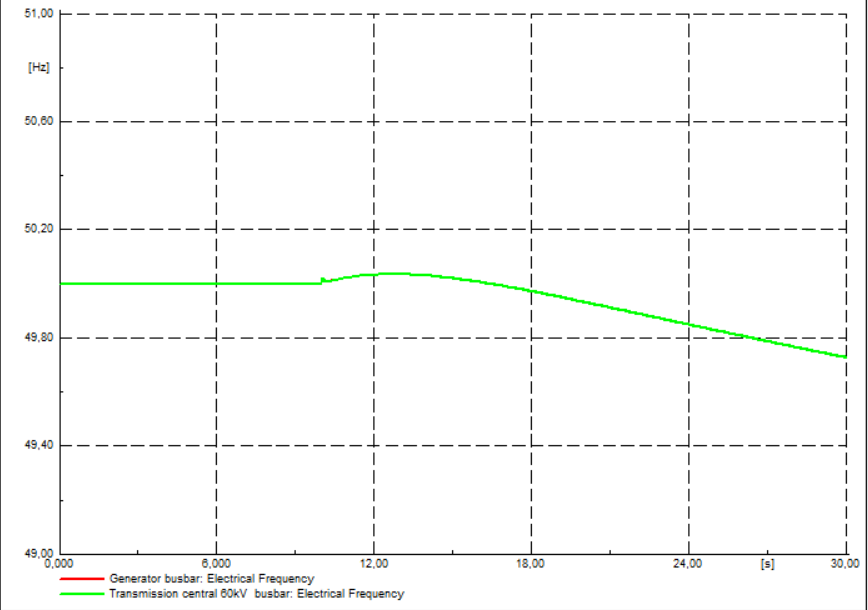
\includegraphics[width=1.00\textwidth]{figurer/LossOfTown/Freq1} % Højre billede
	\end{minipage}
	\\ % Figurtekster og labels
	\begin{minipage}[t]{0.48\textwidth}
		\caption{Case 2, Tilstand 1, Spændingsgraf} % Venstre figurtekst og label
		\label{fig:C2T1V}
	\end{minipage}
	\hfill
	\begin{minipage}[t]{0.48\textwidth}
		\caption{Case 2, Tilstand 1, Frekvensgraf} % Højre figurtekst og label
		\label{fig:C2T1F}
	\end{minipage}
\end{figure}

\textbf{Tilstand 2: Batterierne i alle byer kobles ind 0,5s efter fejlen og absorberer 0,304MW som kompensation for tabet af byen. Alle med pf 0,95}
\begin{figure}[H]
	\centering
	\begin{minipage}[b]{0.48\textwidth}
		\centering
		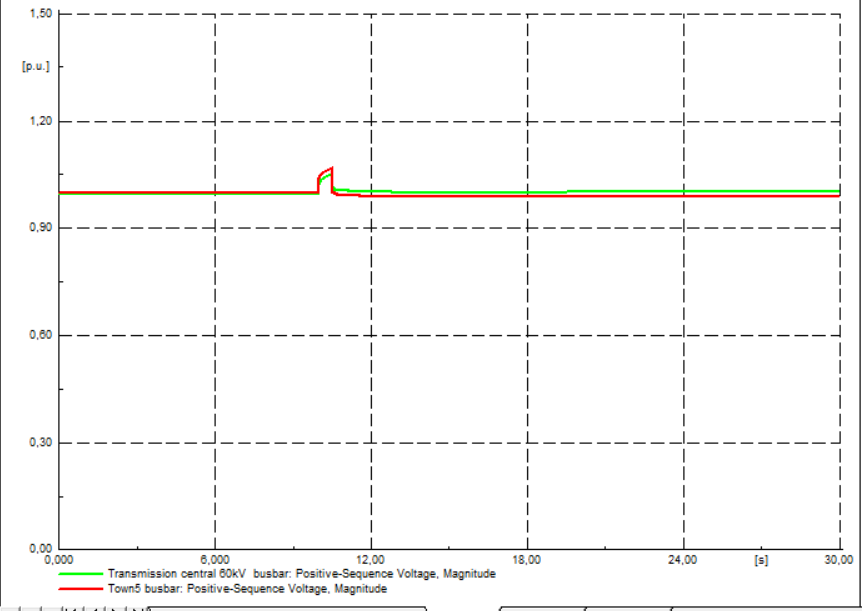
\includegraphics[width=1.00\textwidth]{figurer/LossOfTown/Voltage2} % Venstre billede
	\end{minipage}
	\hfill
	\begin{minipage}[b]{0.48\textwidth}
		\centering
		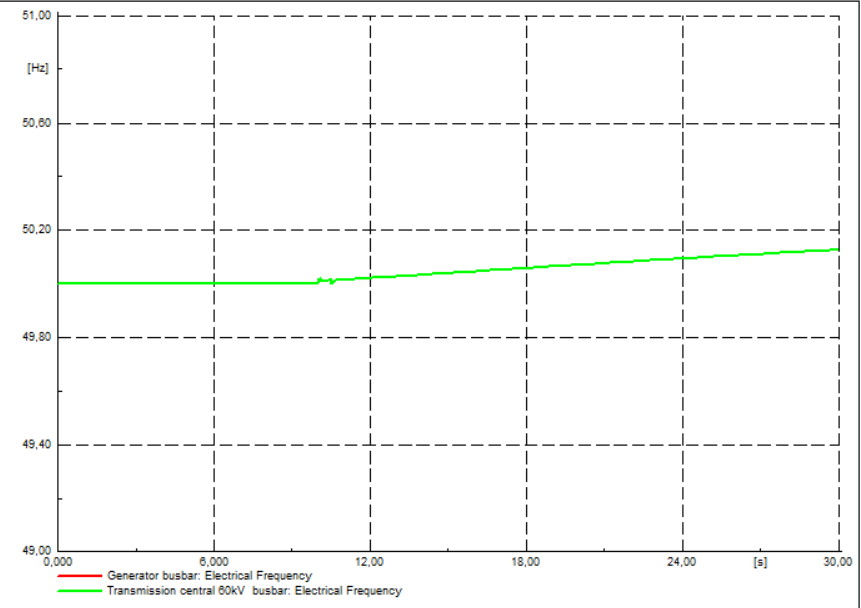
\includegraphics[width=1.00\textwidth]{figurer/LossOfTown/Freq2} % Højre billede
	\end{minipage}
	\\ % Figurtekster og labels
	\begin{minipage}[t]{0.48\textwidth}
		\caption{Case 2, Tilstand 2, Spændingsgraf} % Venstre figurtekst og label
		\label{fig:C2T2V}
	\end{minipage}
	\hfill
	\begin{minipage}[t]{0.48\textwidth}
		\caption{Case 2, Tilstand 2, Frekvensgraf} % Højre figurtekst og label
		\label{fig:C2T2F}
	\end{minipage}
\end{figure}

\textbf{Tilstandsoverblik}
\begin{figure}[H] % (alternativt [H])
	\centering
	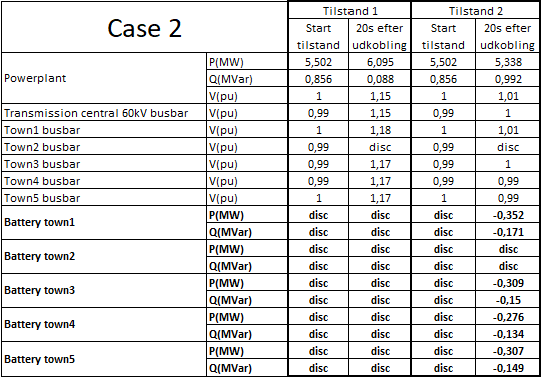
\includegraphics[width=1\textwidth]{figurer/LossOfTown/Overview}
	\caption{Overblik for spænding og effektoverførelse i nettet}
	\label{fig:C2Overview}
\end{figure}

I tilstand 1 ses det at spænding stiger betydeligt ved Town5 busbar og Transmissions central 60kV busbar. I tilstand 2 stiger spændingen kortvarigt indtil batterierne kobles ind. Spænding stiger i tilstand 1 da der er for meget produktion i forhold til belastning. Da batterierne i tilstand 2 påbegynder opladning hurtigt efter tabet af Town2 kompensere de for det manglende belastning og stabilisere derfor spændingen til normal.

Frekvensen starter med at stige lidt pga. den udkoblede belastning. hvorefter den begynder at falde lidt igen. Dette sker formentlig fordi at belastning stiger i de ikke afkoblede byer pga. overspændingen og det ser ikke ud til at Powerfactory tilpasser spændingsniveauet efter at belastningen stiger igen. I tilstand 2 stiger frekvensen formentlig pga. det hurtigt afkoblede produktion og da inertien er ret høj i systemet går der lidt tid inden den tilpasser sig systemet igen.
  
